\documentclass[UTF8]{ctexart}

\usepackage{amsmath}
\usepackage{multicol}
\setlength{\parindent}{2em}
\addtolength{\topmargin}{-54pt}
\setlength{\oddsidemargin}{0.63cm}  % 3.17cm - 1 inch
\setlength{\evensidemargin}{\oddsidemargin}
\setlength{\textwidth}{14.66cm}
\setlength{\textheight}{24.00cm}    % 24.62
\usepackage{graphicx}
\usepackage{float}
\usepackage{multirow}
\usepackage{subfigure}
\begin{document}

%标题
\begin{center}
\Huge\textbf{非线性电路混沌及其同步控制}
\renewcommand{\baselinestretch}{5.0}
\end{center}
\begin{center}
\small
\begin{tabular}{llll}
\textbf{姓名}&李励玮     &\textbf{学号}  &201711140236\\
\textbf{指导老师}&熊俊 &\textbf{实验日期}& 2019.11.15\\
\end{tabular}
\end{center}

%摘要
\small
\noindent\textbf{摘要}:实验运用三段分段线性有源非线性负阻元件,搭建蔡氏电路,输出混沌信号。混沌有别于噪音,具有两个特征,费根鲍姆常数和奇异吸引子,可以利用非线性电路测量准费根鲍姆常数并观察倍周期分岔和奇异吸引子。利用非线性电路的混沌同步现象可以实现混沌通信,混沌通信具有保密性强的特点。
\newline\textbf{关键字:负阻;非线性电路;费根鲍姆常数;倍周期分岔;奇异吸引子;混沌同步;混沌通信}

~\\

\begin{multicols}{2}
%引言
\section{引言}
混沌是非线性动力学系统所特有的运动形式。混沌是由确定性系统产生的随机现象,表现为系统相空间轨道呈现出高度不稳定性,系统行为对初始条件有敏感性(蝴蝶效应)。但由于系统的确定性決定了这是一种内在的随机性,混沌不等于无序。

由于电路可以用精密的元器件控制,目前最丰富的混沌现象是在非线性振荡电路中观察到。蔡氏电路是能产生混沌行为的最简单的电路,通过蔡氏电路参数的改变可以实现倍周期分岔到混沌,再到周期窗口的全过程。

混沌信号具有宽频谱、类噪声、容易产生和料确再生等特性,非常适合于保密通信,使得混沌在保密通信中具有较好的前景,而同步技术的发展,为混沌保密通信奠定了基础。


\section{实验目的}
学习有源非线性负阻元件的工作原理,借助蔡氏电路掌握非线性动力学系统运动的一般规律,了解混沌同步和控制的基本概念,了解混沌通信原理。

\section{实验原理}
\subsection{倍周期分岔与费根鲍姆常数}
在许多非线性系统中,既有周期运动,又有由于内部的非线性作用产生的混沌运动。倍周期分岔是系统由定态过渡到混沌最重要的途径。
\newline\textbf{倍周期分岔}:周期不断加倍直至出现混沌。
\newline\textbf{费根鲍姆常数}:动力学系统中分盆点处参量$\mu$的取值$\mu_n$的收敛服从普适规律,即存在非线性参数
\begin{equation}
\delta_{n}=\frac{\mu_{n}-\mu_{n-1}}{\mu_{n+1}-\mu_{n}}
\end{equation}
,而$\delta=\lim _{n \rightarrow \infty} \delta_{n}=4.6992016091029$,$\delta$为费根鲍姆常数。出现倍周期分岔预示着混沌的存在,换句话说,对于任何一个混沌系统都存在着常数$\delta$。

\subsection{有源非线性负阻}
负阻:当电阻的端电压增加时,流过电阻的电流减小,表现为I-U特性曲线斜率的倒数$\frac{\Delta U}{\Delta I}$为负。
自然界中不存在负阻元件,只有当电路上有电流流过时,才会产生负阻。负阻元件的实现方法有多种,一种常见的实现负阻的电路由正阻和运算放大器构成一个负阳抗变换器电路。由于运算放大器工作需要有一定的工作电压,因此,这种负阻称为有源负阻。等效电路如图:
\begin{figure}[H]
\centering
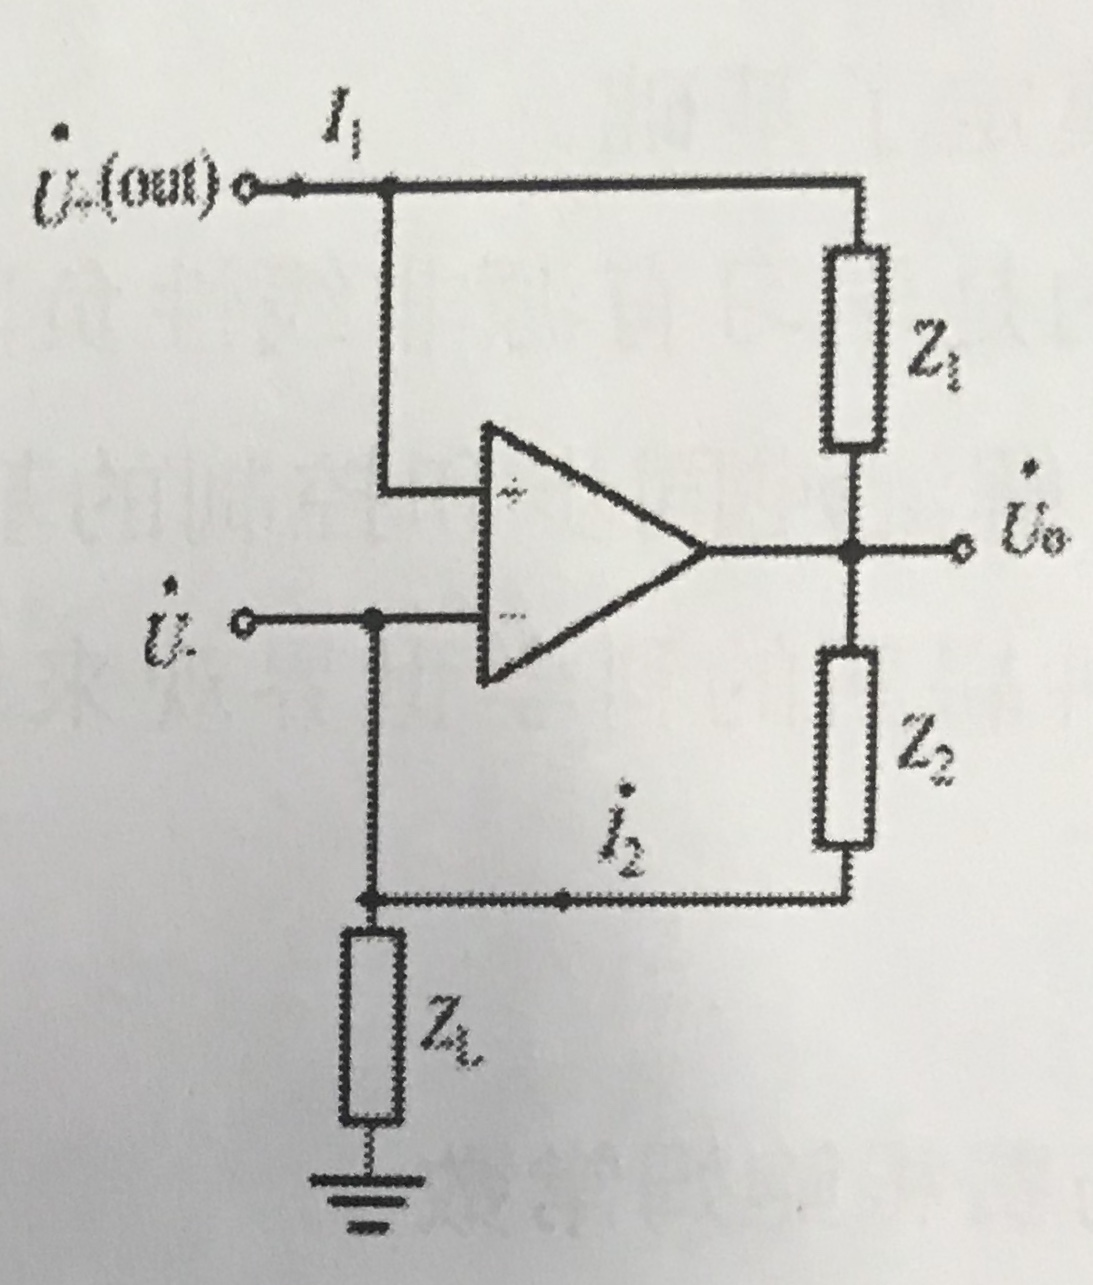
\includegraphics[width=3cm]{2.jpg}
\caption{等效电路}
\end{figure}
它可以等效于一个有载二端口网络,其输入阻抗$Z_N$是指从输入端看进去的阻抗。假设运算放大器是理想的,则$U_{+}=U_{-}$,由于$I_1Z_1=-I_2Z_2$,故输入阻抗为
\begin{equation}
Z_N=\frac{U_+}{I_1}=-\frac{Z_1}{Z_2}\frac{U_+}{I_2}=-\frac{Z_1}{Z_2}Z_L
\end{equation}
若$Z_1=Z_2$,则$Z_N=-Z_L$。这就是说,当负载端接入任意一个无源电阻时,在有源端(激励端)就得到一个负阻元件。本实验所用的负阻为三段分段线性有源非线性负阻元件,$I-U$ 特性曲线分成五个折线段,只有中间的三段折线区域可以产生负阻效应。

\subsection{非线性电路}
\begin{figure}[H]
\centering
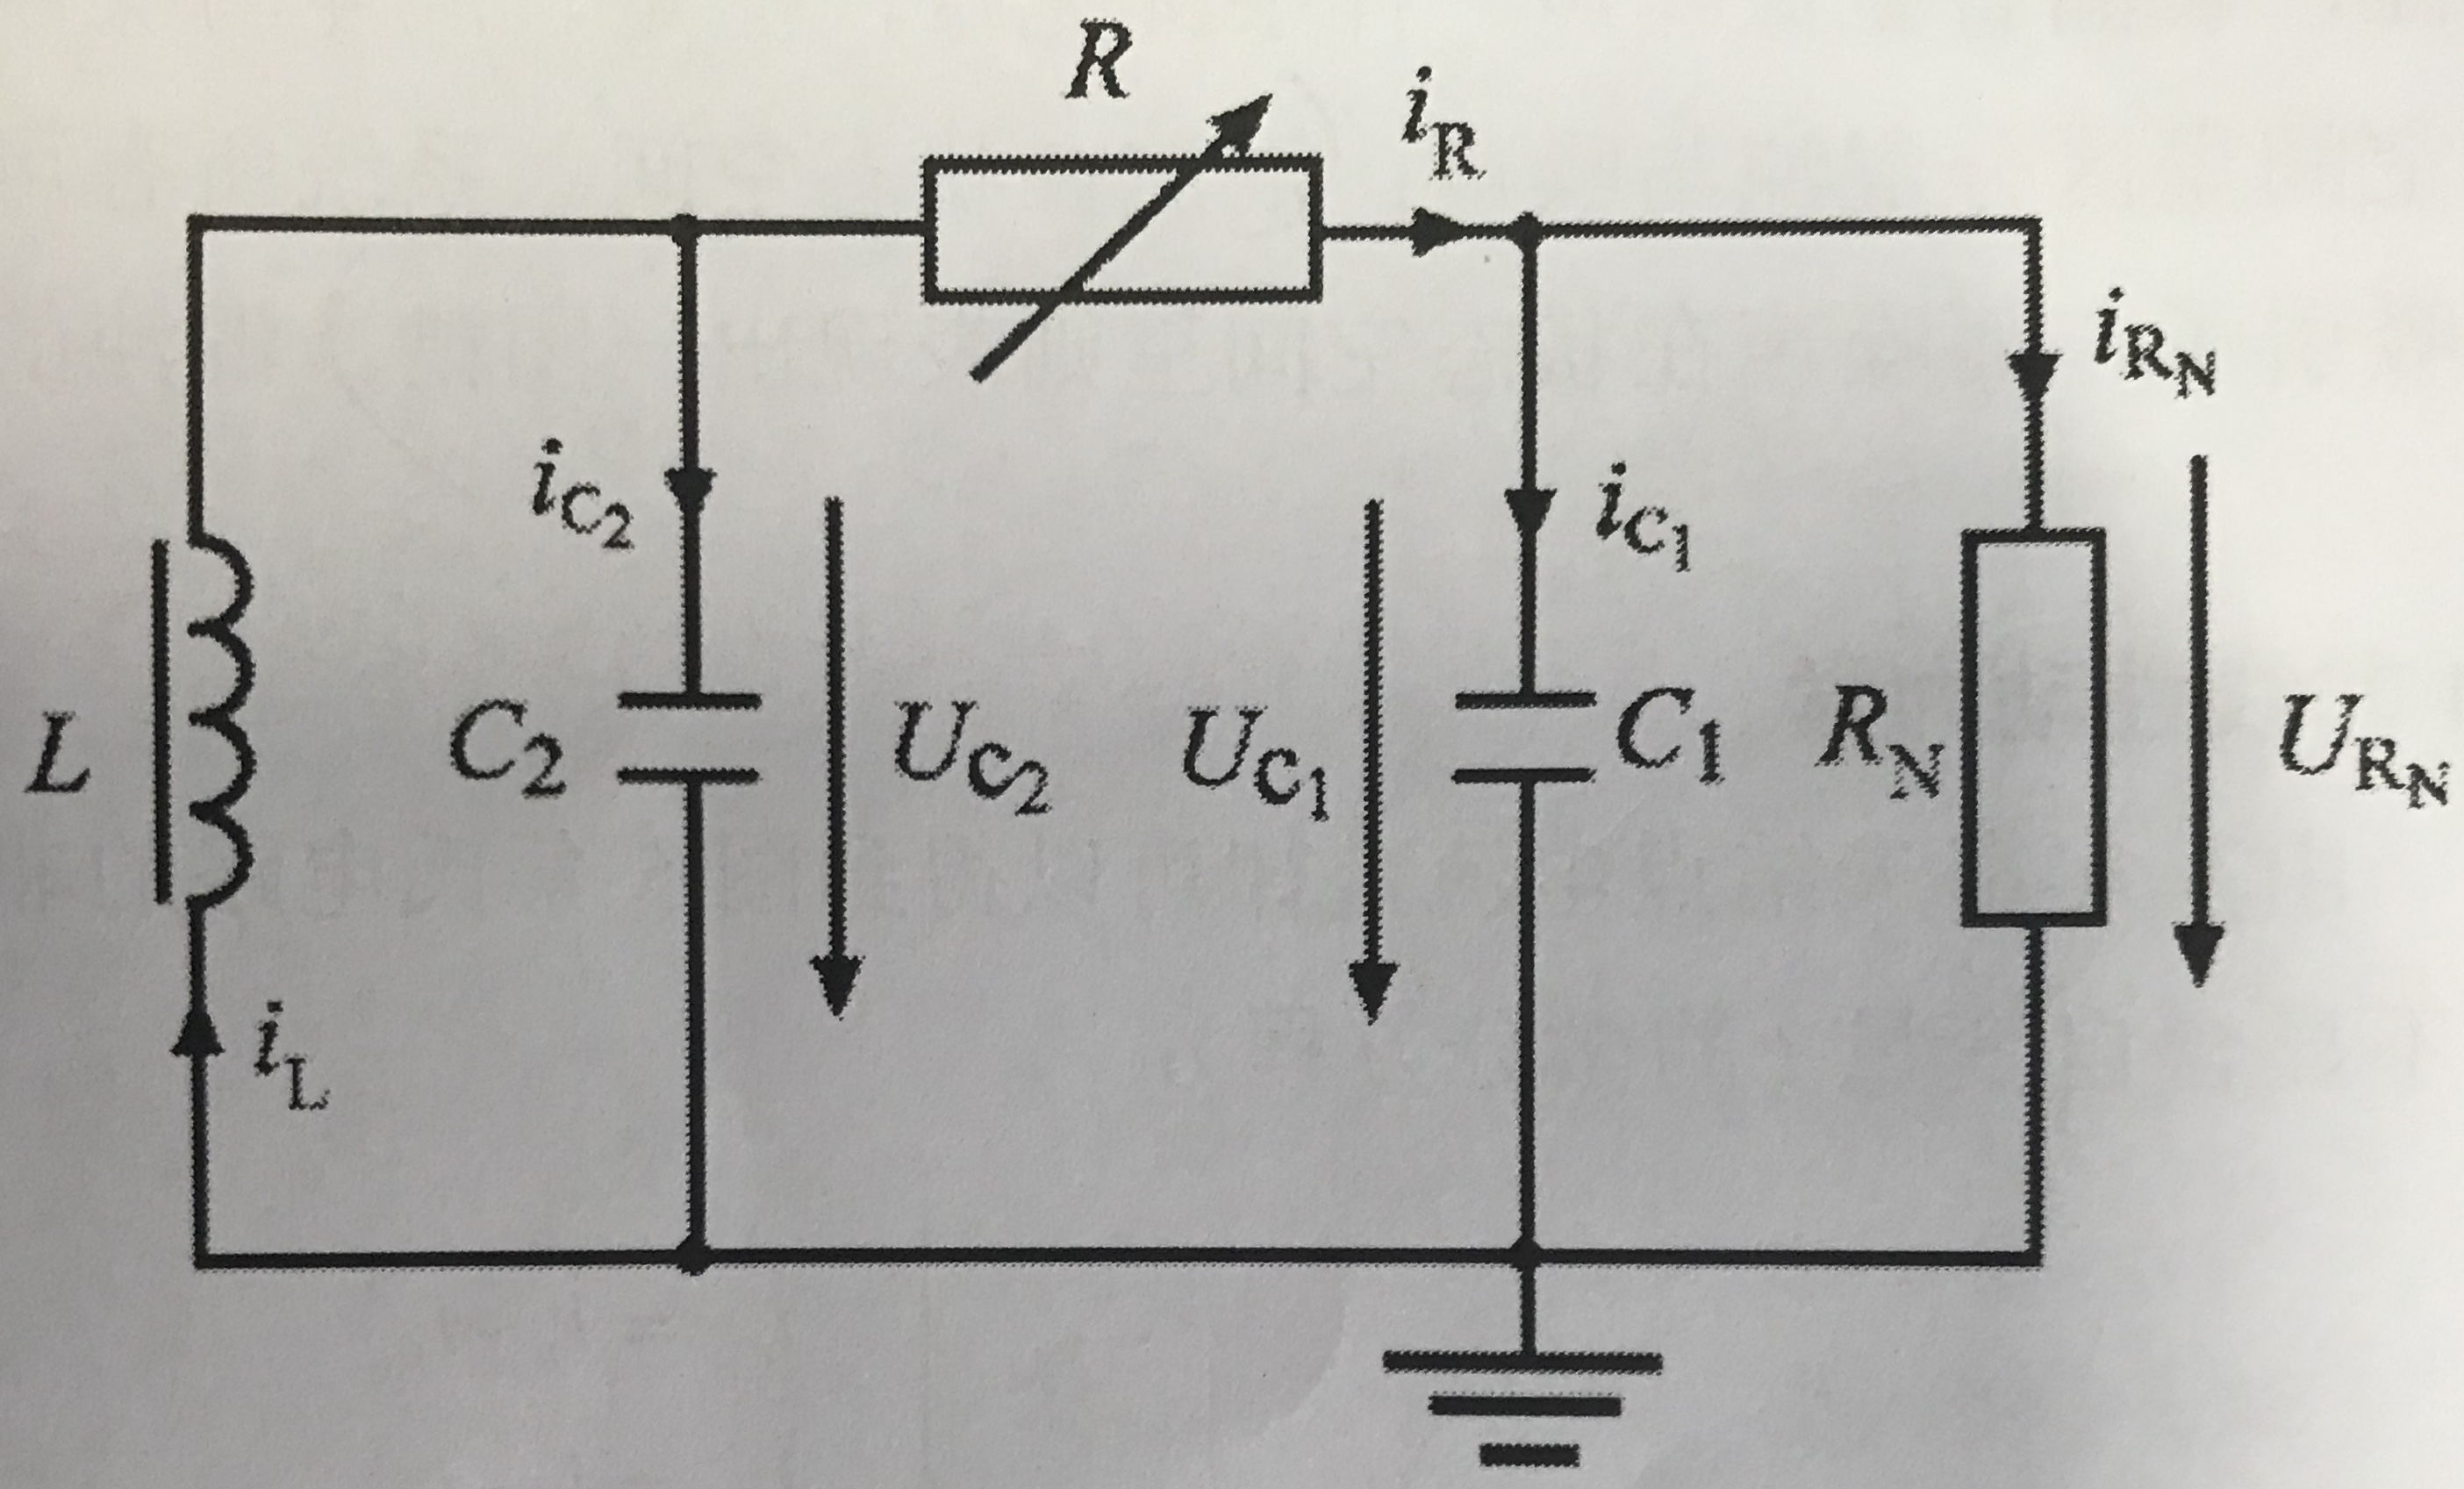
\includegraphics[width=5cm]{5.jpg}
\caption{蔡氏振荡电路}
\end{figure}
如图2为一个典型的蔡氏电路,其中$R_N$有两个作用,一是电路的损耗电阻被抵消使得输出电流维持LC振荡器等幅振荡;二是最重要的,使振荡周期产生分岔和混沌等一系列非线性现象。$R_N$是非线性电路的核心器件,是电路系统产生非线性运动的必要条件。$R_x$中的双运放TL082的前级和后级正负反馈同时存在,当正反馈大于负反馈时,振荡电路才能振荡。因此,正反馈成为如图2所示振荡型非线性电路的必要条件。

参量$R$、$L$、$C_1$和$C_2$的取值洪定了蔡氏电的初始条件,也将导致电路的不同运动形式,周期振、倍周期分岔或者混沌等。非线性系的运动状态可以用相图法进行分析。
\newline\textbf{相图}:假设描写系统状态的量为$U$,$\dot{U}=\frac{dU}{dt}$,那么$U$与$\dot{U}$构成的二维图形叫相图。在相图中的每一条闭合曲线代表系统运动的一个轨迹。

由实验结果还可以发现混沌的另一个特征:局域看,系统每一次运动轨迹都不重复,表现出随机性和不稳定性。但是,全局看,所有的轨迹最终都被捕捉到一个不变的集合,即奇怪吸引子。奇怪吸引子的形成表明混沌有某种确定性和稳定性。借助奇怪吸引子在状态空间里可以区分混沌与噪声。

\subsection{非线性动力学}
由基尔霍夫结点电流定律可以得到图2蔡氏电路的非线性动力学方程,它是一个三阶自治方程(不显含自变量$t$的微分方程)
\begin{equation}
\left\{\begin{aligned} C_{1} \frac{\mathrm{d} U_{C_{1}}}{\mathrm{d} t} &=\frac{1}{R}\left(U_{C_{2}}-U_{C_{1}}\right)-\frac{1}{R_{\mathrm{N}}\left(U_{C_{1}}\right)} U_{C_{1}} \\ C_{2} \frac{\mathrm{d} U_{C_{2}}}{\mathrm{d} t} &=\frac{1}{R}\left(U_{C_{1}}-U_{C_{2}}\right)+i_{L} \\ L \frac{\mathrm{d} i_{L}}{\mathrm{d} t} &=-U_{C_{2}} \end{aligned}\right.
\end{equation}
式中,$R_N(U_{C_1})$是非线性负阻;由于$U_{R_N}=U_{C_1}$,$R_N$是$U_{C_1}$的函数。由于$U_{C_1}$在每个区域上的取值不同,故方程组(3)中的每个方程都是非线性的。且每一个方程表示动力系统每一个状态变量随时间的变化率;方程形式不会随时间变化,表明系统动力学规律的不变性。
方程组(3)中的$U_{C_{1}}$、$U_{C_{2}}$和$i_{L}$任一均可描述系统的运动状态;且参量$L$、$R$、$C_1$和$C_2$的取值对计算结果影响极大。

\subsection{混沌同步}
\textbf{混沌同步}:一个系统的混沌动力学轨道收敛于另一个系统的混沌动力学轨道,以致在以后的时间里两个系统始终保持步调一致。

驱动——响应方法是混沌同步的重要方法,它将系统分成两个子系统:驱动子系统和响应子系统然后对响应子系统进行复制,并用驱动子系统产生的信号驱动该复制的系统。混沌同步是为了在个相同的具有任意初始件的响应系统中,从一个驱动系统中恢复给定的混轨迹。

实验中由两个相同的蔡氏电路和一个单向耦合系统构成。相同的蔡氏电路是指两个电路的元件的参数尽可能的接近,这是确保混沌同步能够实现的基本条件。单向耦合系统由一个运算放大器和一个可调电阻$R_c$构成。
\newline\textbf{单向}:驱动系统只对响应系统产生作用,而响
应系统不能对驱动系统作用。

驱动系统$C_1$两端的电压信号通过运算放大器等值地传输到单向耦合系统中的$R_c$左侧。由于单向耦合系统,响应系统的运动状态不能影响驱动系统。这样,$R_c$的左右两端分别得到驱动系统的$C_1$信号和响应系统的$C_2$信号。驱动系统和响应系统不同步时,$C_1$、$C_2$不等,可以调节$R_c$实现相等。

\subsection{混沌通信}
混沌通信的基本思想是将要传输的信号混入混沌信号中进行传输,然后在接收端通过减去混沌信号得到所需信号。由于传输的是用混沌信号掩盖过的混合信号,所以混沌通信保密性强。本实验设计的混沌通信电路由驱动系统、响应系统、单向耦合系统、加法器和减法器组成。

实现通信的方法:调节驱动系统和响应系统出现混沌状态;调节使驱动和响应系统同步;使要传输的信号,通过加法器与驱动系统混沌信号混合后进行传输,在接收端用减法器将传输信号与响应系统混沌信号相减。由于响应系统与驱动系统同步,故相减的结果为所需的信号。由于噪声的影响和电路损耗,输出信号与输入信号不完全相同,可以在减法器后接一个滤波器,减小输出信号的噪声。

\section{实验内容}
\noindent\textbf{1.测量非线性电阻的I-U特性曲线}

自己设计并搭建测量电路(用电阻箱)。
\newline\textbf{2.观察并记录当电阻变化时非线性电路的运动状态}

搭建非线性电路。将$C_1$、$C_2$上的电压信号接数字示波器上的CH1、CH2通道,选择示波器xy显示模式,适当选择数字示波器长余辉模式。

单调改变可变电阻$R$,用数字示波器(借助 Open Wave-2KE软件)记录系统的8种不同状态:1P→2P→4P→8P→阵发混沌→3P窗口→单吸引子→不稳定双吸引子,同时用示波器测量非线性负阻两端电压。确定不同的状态在非线性负阻I-U分段折线上的区域,即确定本实验非线性负阻的工作区域。
\newline\textbf{3.测量准费根鲍姆常数}

利用电容箱单调改变C2,测量准费根鲍姆常数。
\newline\textbf{4.混沌同步实验}

搭建混沌同步电路,将其中一个蔡氏电路作为驱动系统,另外一个蔡氏电路作为响应系统。分别调节可变电阻,使得两个蔡氏电路处于大致相同的双吸引子状态,用两个模拟示波器观察。采用隔离器和耦合电阻将两个蔡氏电路连接起来。将C1、C1上的电压信号分别接数字示波器上的CH1、CH2通道。

分别调节驱动系统和响应系统中的可变电阻、改变耦合电阻,观察电路的变化,记录混沌同步、准同步和去同步状态。
\newline\textbf{5.加密通信}

在混沌同步的基础上做本实验。将信号源输出的正弦波信号输入到加法器的加密信号端,将驱动系统的混沌信号加到加法器的混沌信号端,加法器的输出端信号输入至减法器中的混合信号端,记录输入正弦波、混沌信号、加密信号、滤波器前信号和滤波后信号,说明混沌加密通信原理。


\end{multicols}

\section{实验结果分析与讨论}
\noindent\textbf{1.测量非线性电阻的I-U特性曲线}
\begin{table}[H]
\tiny
\centering
\begin{tabular}{|l|l|l|l|l|l|l|l|l|l|}
\hline
$U$/$V$  & 12.40 & 11.92 & 11.52 & 10.96 & 10.50 & 10.285 & 9.97  & 9.59  & 8.93  \\ \hline
$I$/$mA$ & 0.155 & 1.32  & 2.3   & 3.6   & 4.76  & 4.89   & 4.76  & 4.61  & 4.34  \\ \hline
$U$/$V$  & 8.58  & 8.08  & 7.50  & 7.00  & 6.55  & 6.04   & 5.50  & 5.01  & 4.50  \\ \hline
$I$/$mA$ & 4.19  & 3.97  & 3.73  & 3.52  & 3.33  & 3.11   & 2.88  & 2.68  & 2.47  \\ \hline
$U$/$V$  & 4.03  & 3.50  & 3.01  & 2.53  & 2.03  & 1.53   & 0.51  & 0.107 & 0.05  \\ \hline
$I$/$mA$ & 2.27  & 2.05  & 1.85  & 1.65  & 1.45  & 1.32   & 0.395 & 0.088 & 0.045 \\ \hline
\end{tabular}
\end{table}
\begin{figure}[H]
\centering
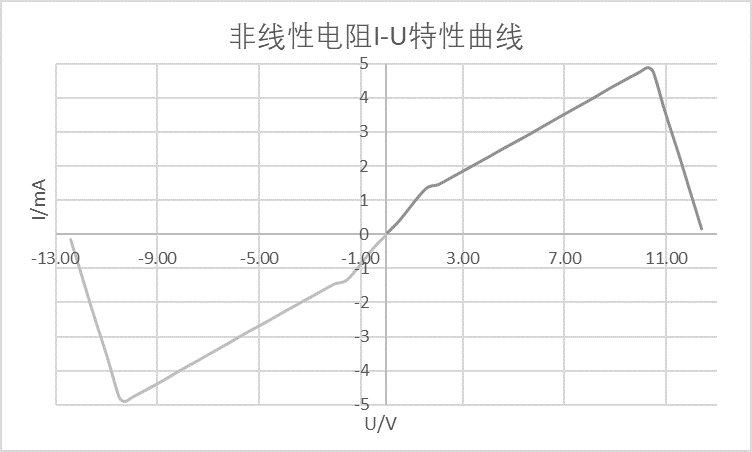
\includegraphics[width=10cm]{U-I.png}
\end{figure}
可见I-U特性曲线分成五个折线段。其中间的三段可见,当加在此元件上的电压增加时,通过它的电流却减小,产生负阻效应。

~\\
\noindent\textbf{2.观察并记录当电阻变化时非线性电路的运动状态,记录系统的8种不同状态:}
\begin{figure}[H]
\centering
  \subfigure[1P]{ 
    \label{fig:subfig:a} %% label for first subfigure 
    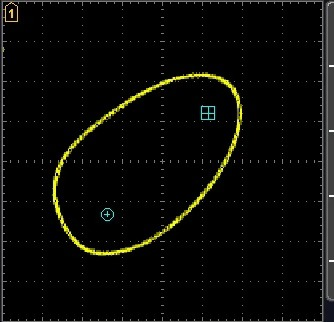
\includegraphics[width=3.3cm]{1p.jpg}} 
  \subfigure[2P]{ 
    \label{fig:subfig:b} %% label for second subfigure 
    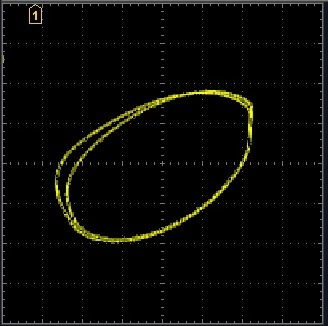
\includegraphics[width=3.3cm]{2p.jpg}} 
  \subfigure[4P]{ 
    \label{fig:subfig:c} %% label for second subfigure 
    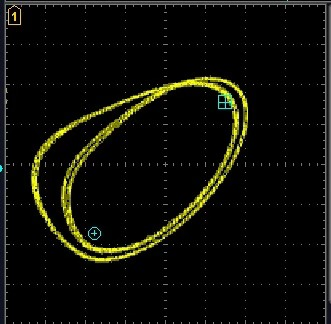
\includegraphics[width=3.3cm]{4p.jpg}} 
  \subfigure[8P]{ 
    \label{fig:subfig:d} %% label for second subfigure 
    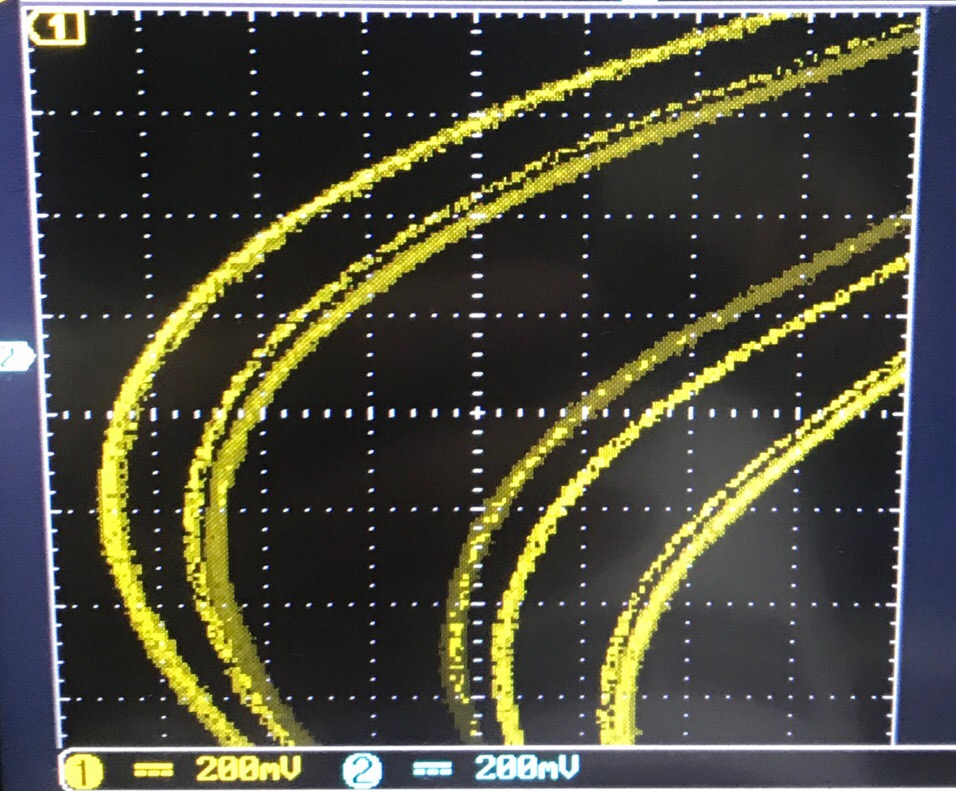
\includegraphics[width=3.3cm]{8p.jpg}}
  \subfigure[3P]{ 
    \label{fig:subfig:e} %% label for second subfigure 
    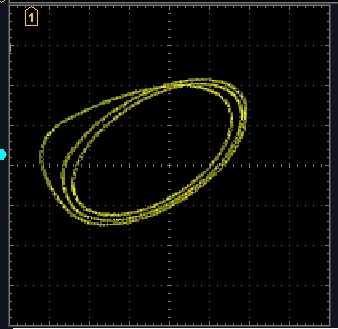
\includegraphics[width=4.5cm]{3p.jpg}} 
  \subfigure[单吸引子]{ 
    \label{fig:subfig:f} %% label for second subfigure 
    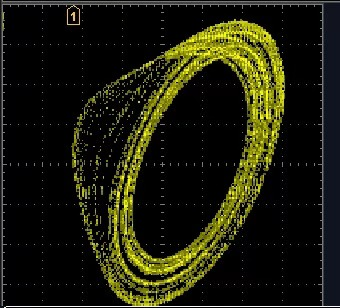
\includegraphics[width=4.5cm]{single.jpg}}
  \subfigure[不稳定双吸引子]{ 
    \label{fig:subfig:g} %% label for second subfigure 
    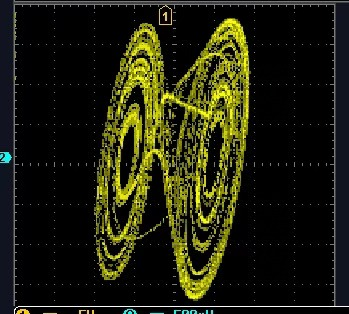
\includegraphics[width=4.5cm]{double.jpg}}
\end{figure}
由图可见,系统的周期不断加倍最后出现混沌现象,因此倍周期分岔可以使系统由定态过渡到混沌;另一方面,、所有的轨迹最终都被捕捉到一个不变的集合,即奇怪吸引子,可见混沌有某种确定性和稳定性。

~\\
\noindent\textbf{3.观察并记录当电容C2变化时非线性电路的运动状态,计算准费根鲍姆常数}
\begin{table}[H]
\centering
\tiny
\begin{tabular}{|l|l|l|l|}
\hline
状态          & 1P→2P   & 2P→4P   & 4P→8P   \\ \hline
$C_2/\mu F$ & 0.05420 & 0.05628 & 0.05687 \\ \hline
\end{tabular}
\end{table}
计算得准费根鲍姆常数
$\delta =\frac{\mu_{n}-\mu_{n-1}}{\mu_{n+1}-\mu_{n}}=4.74576271$。与费根鲍姆常数有差异的原因是这里仅仅是分岔使较早期的记录;另一方面是记录的转变时对应的$C_2$是由人眼判断的,存在一定误差。

~\\
\newline\textbf{4.混沌同步实验}
\begin{figure}[H]
\centering
 \subfigure[同步]{ 
    \label{fig:subfig:a} %% label for second subfigure 
    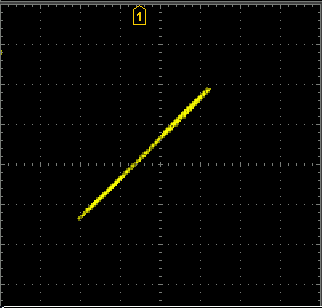
\includegraphics[width=4.5cm]{synchronous.png}} 
  \subfigure[准同步]{ 
    \label{fig:subfig:b} %% label for second subfigure 
    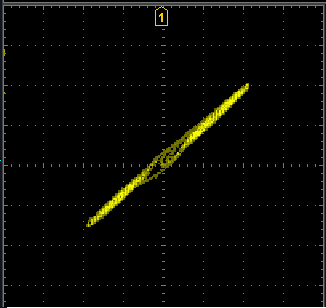
\includegraphics[width=4.5cm]{quasi-synchronous.png}}
  \subfigure[去同步]{ 
    \label{fig:subfig:c} %% label for second subfigure 
    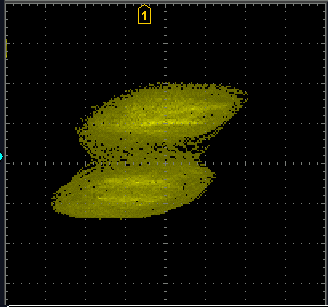
\includegraphics[width=4.5cm]{desynchronous.png}}
\end{figure}

~\\
\noindent\textbf{5.加密通信}
\begin{figure}[H]
\centering
 \subfigure[输入正弦波]{ 
    \label{fig:subfig:b} %% label for second subfigure 
    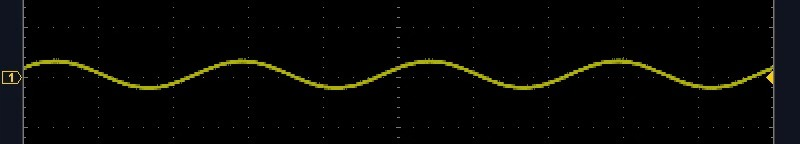
\includegraphics[width=7.1cm]{input.jpg}} 
  \subfigure[混沌信号]{ 
    \label{fig:subfig:b} %% label for second subfigure 
    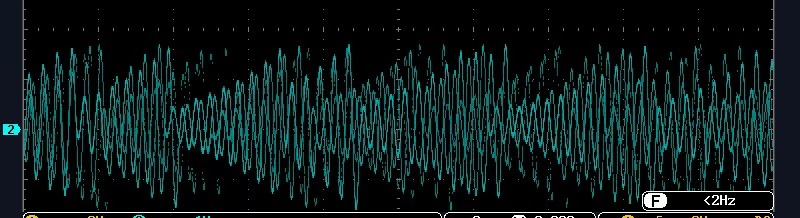
\includegraphics[width=7.1cm]{chaos.jpg}}
  \subfigure[加密信号]{ 
    \label{fig:subfig:b} %% label for second subfigure 
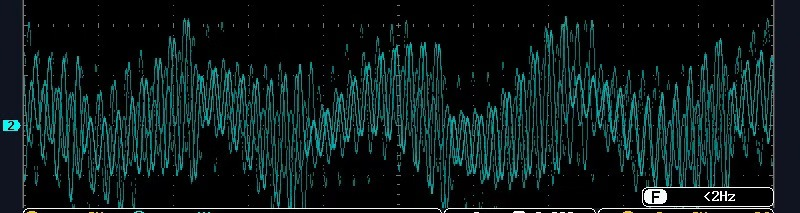
\includegraphics[width=7.1cm]{mixed.jpg}}
  \subfigure[滤波器前信号]{ 
    \label{fig:subfig:b} %% label for second subfigure 
    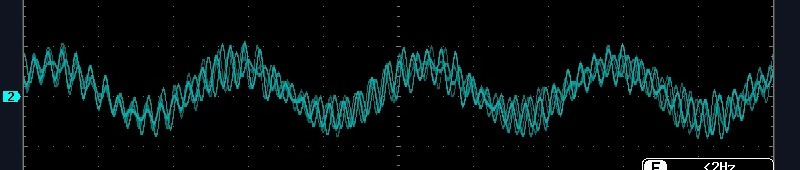
\includegraphics[width=7.1cm]{before-smoothing.jpg}}
  \subfigure[滤波后信号]{ 
    \label{fig:subfig:b} %% label for second subfigure 
    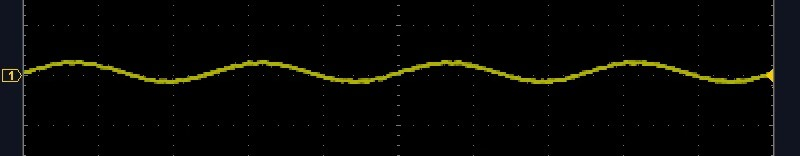
\includegraphics[width=7.1cm]{after-smoothing.jpg}}
\end{figure}
混沌加密通信原理:将要传输的信号混入混沌信号中进行传输,然后在接收端通过减去混沌信号得到所需信号。由于传输的是用混沌信号掩盖过的混合信号,所以混沌通信保密性强。

\section{结论}
负阻元件中当电阻的端电压增加时,流过电阻的电流减小,实验所用的负阻原件是三段分段线性有源非线性负阻元件。非线性电路可以产生混沌信号,混沌具有两个特征,费根鲍姆常数和奇异吸引子,有别于噪音。利用非线性电路的混沌同步现象可以实现混沌通信,混沌通信具有保密性强的特点。

\section{参考文献}
\small
\noindent[1]北师大物理实验教学中心,近代物理实验2讲义p17-24,2019.

\begin{figure}[H]
\centering
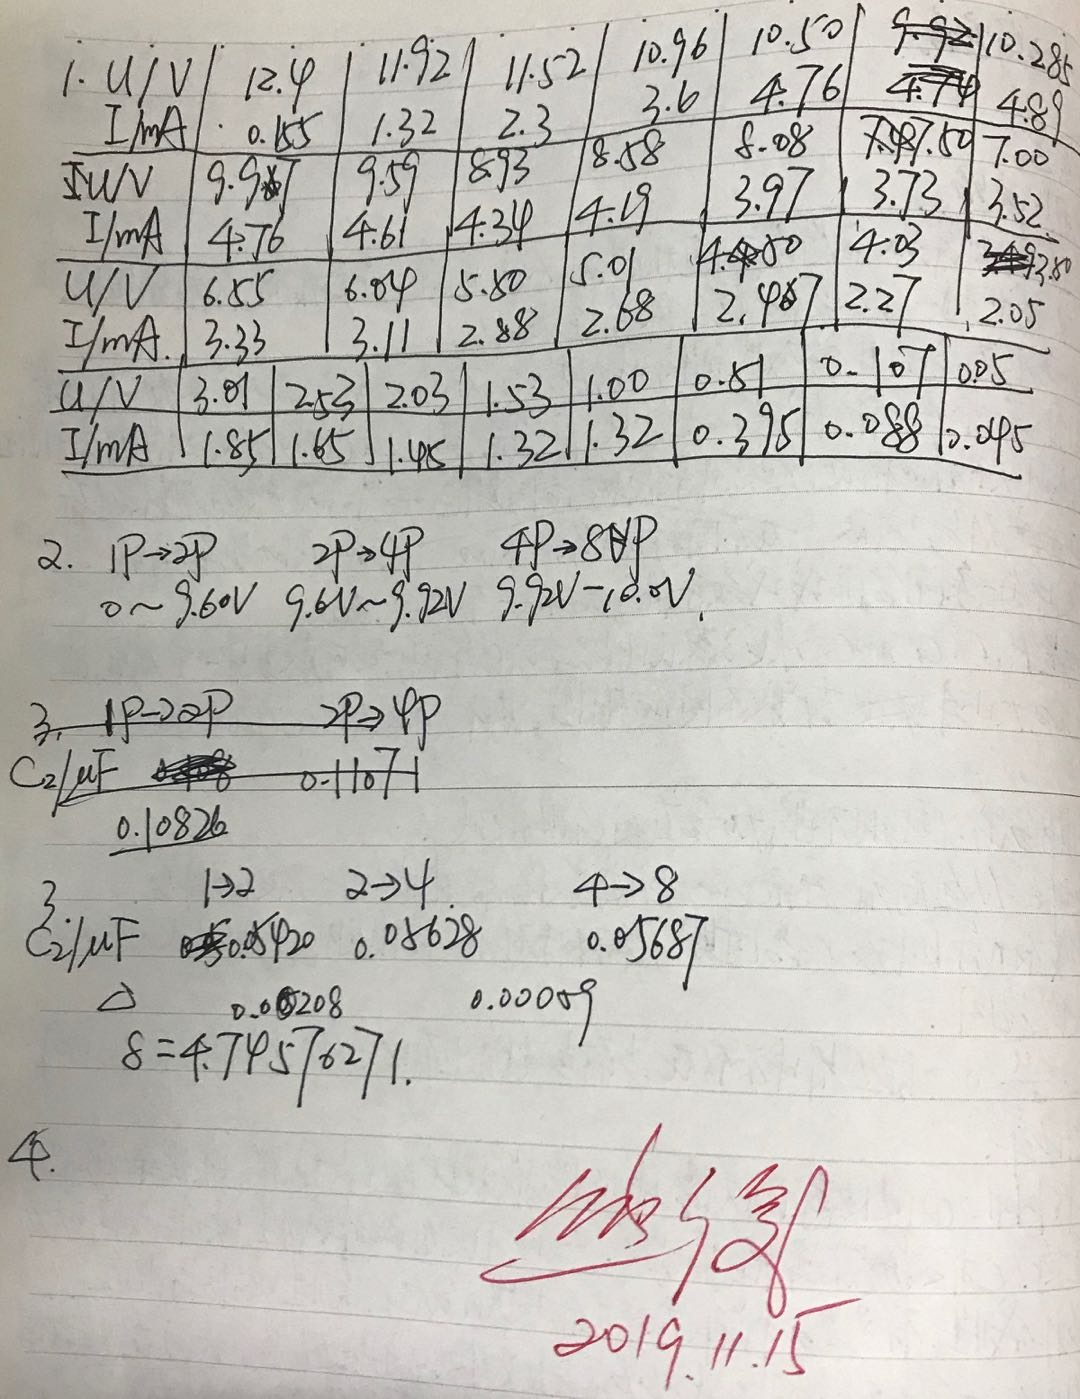
\includegraphics[width=7cm]{record.jpg}
\end{figure}
\end{document}